%!TEX TS-program = xelatex
%!TEX encoding = UTF-8 Unicode

\documentclass[12pt,letterpaper]{article}
\usepackage{fontspec}
\usepackage{geometry}
\geometry{letterpaper, textwidth=6.5in, textheight=9.5in, marginparsep=20pt, marginparwidth=2in}
\setlength\parindent{0in}
\usepackage[usenames,dvipsnames]{color}

% math packages
\usepackage{amsmath}
\usepackage{arevmath}
\usepackage{enumerate}

% for sans serif math
%\usepackage{cmbright}

\usepackage{cancel}
% alp's math bold command: Use it like \mb{\lambda} or \mb{X}.
\DeclareRobustCommand{\mb}[1]{\ensuremath{\boldsymbol{\mathbf{#1}}}}

% cond. independence
\newcommand\independent{\protect\mathpalette{\protect\independenT}{\perp}}
\def\independenT#1#2{\mathrel{\rlap{$#1#2$}\mkern2mu{#1#2}}}



\usepackage{xunicode}
\usepackage{xltxtra}
\defaultfontfeatures{Mapping=tex-text,Ligatures=Common, Scale=1}
%\setromanfont [Ligatures={Common}, Numbers={OldStyle}, Variant=01]{Hoefler Text Roman}
%\setromanfont{Whitney HTF Light}
%\setmainfont{Whitney HTF}
\setmainfont[
 BoldFont={Whitney HTF Medium},
 ItalicFont={Whitney HTF Light Italic},
 BoldItalicFont={Whitney HTF Medium Italic}
 ]{Whitney HTF}
\usepackage[]{hyperref}
\usepackage[
    style=numeric-comp,
    sorting=none,
    doi=false,
    isbn=false,
    url=true,
    eprint=false,
    natbib=true,
    maxnames=99
]{biblatex}
\addbibresource{Untitled.bib}

\usepackage{dsfont}



%% Commands
\newcommand{\be}{\begin{equation*}}
\newcommand{\ee}{\end{equation*}}
\newcommand{\ba}{\begin{align*}}
\newcommand{\ea}{\end{align*}}
\newcommand{\indicator}{\mathds{1}}

\title{User-artist-song Model (draft)}
\author{Jaan Altosaar, Laurent Charlin, David Blei}

\begin{document}

\makeatletter

\def\maketitle{%
\begin{centering}
\textbf{\large\@title}\\%
\@author\\%
{\today}\\
\end{centering}
\par}

\makeatother
\maketitle
\vspace{10mm}

\section{Motivation}

Listening to music is different than reading articles. The artist of a song is of higher importance than the author of a scientific paper for a given user perusing their library.


We aim to capture this intuition using latent variables representing artist-level topics $\beta_a$, song-level topics $\beta_s$, and user preferences $x_u$ as shown in Figure \ref{fig:uasmodel}.  This model can be extended, for example by connecting the artist-level $\beta_a$ node to the song-level $\beta_s$ node, or the artist-level rating $r_{ua}$ to the song-level rating $r_{uai}$.

% user artist song model
\begin{figure}[htb]
  \begin{center}
    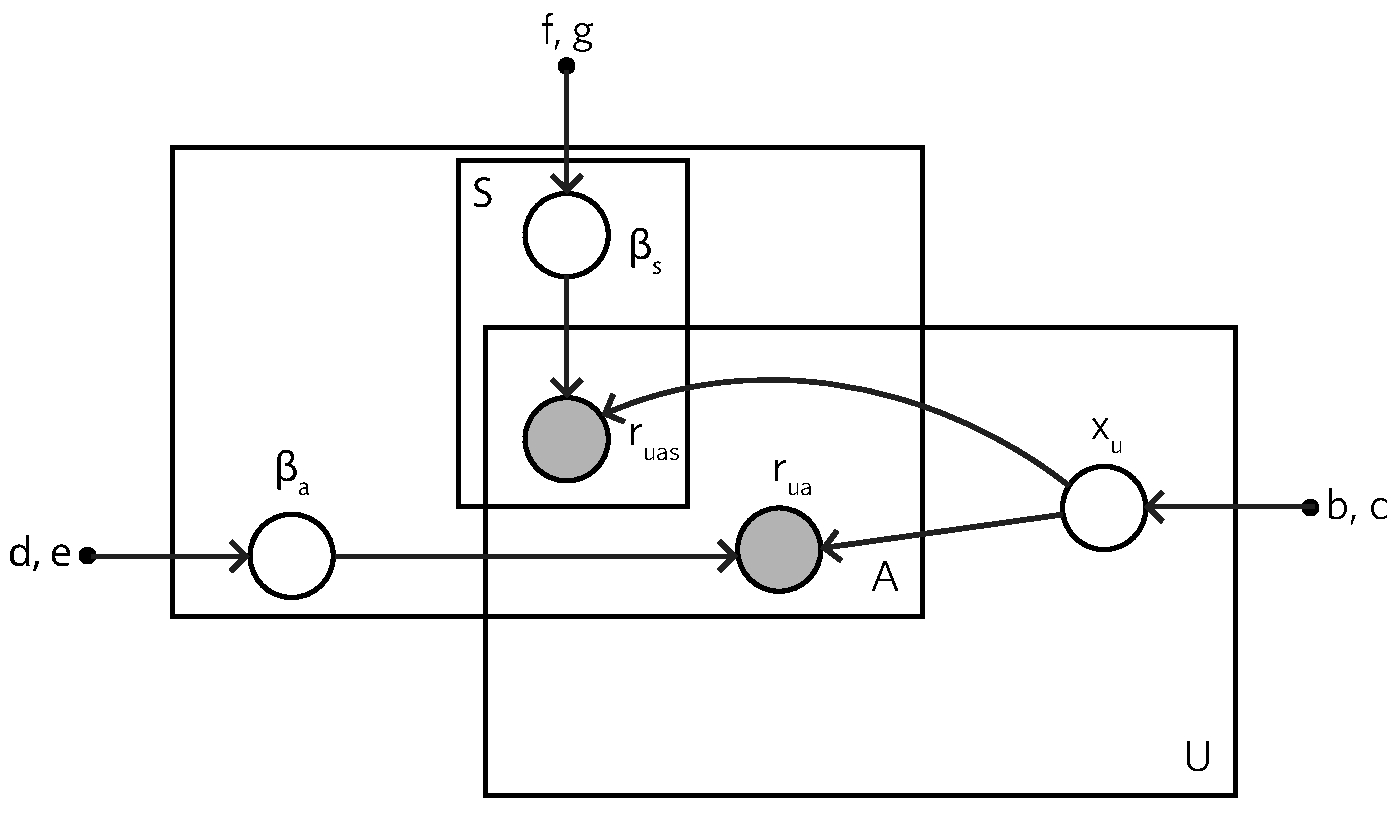
\includegraphics[height=0.5\textwidth]{../fig/user-artist-song-model}
  \end{center}
  \caption{The graphical representation of the user-artist-song model, for $U$ users listening to $A$ artists, and each artist having $S$ songs.}
  \label{fig:uasmodel}
\end{figure}
\clearpage
\section{Generative Process}

The generative process for the observed ratings is partially inspired by content-based Poisson factorization \parencite{Gopalana}:

\begin{enumerate}
\item Draw user preferences $x_u \sim \textrm{\bf Gamma}(b,c)$
\item Draw artist-level topics $\beta_a \sim \textrm{\bf Gamma}(d,e)$
\item Draw song-level topics $\beta_i \sim \textrm{\bf Gamma}(f,g)$
\item Draw user-artist rating $r_{ua} \sim \textrm{\bf Poisson}(x_u^T \beta_a)$
\item Draw user-song rating $r_{uai} \sim \textrm{\bf Poisson}(x_u^T(\beta_a + \beta_i))$
\end{enumerate}

\section{Inference}

Structured Stochastic Variational Inference (SSVI) was recently introduced \parencite{Hoffman2014} as a method to add some dependencies between global and local parameters (as opposed to mean-field inference where there are no such dependencies). Here we derive SSVI first for Poisson factorization \citep{Gopalan2013}, and then for the user-artist-song model (Figure \ref{fig:uasmodel}).

\section{Experiments}

SSVI was used to fit Poisson factorization to the million song data set \citep{Liang2014}. The precision was 8.5\% (compared to 5.2\% for content-based Poisson factorization from last semester).

\printbibliography

\end{document}

%%% Local Variables:
%%% mode: tex-pdf
%%% TeX-master: t
%%% End:
